%------------------------------%
%% ✎ Dylan (V1) %%%%%%%%% ✅ %%
%% ✎ Alain (V2) %%%%%%%%% ✅ %%
%% ✎ Dylan (V3) %%%%%%%%% ✅ %%
%------------------------------%

\afterpage{%
\afterpage{%

    % Arrière-plan conclusion generale
    \AddToShipoutPictureBG*{%
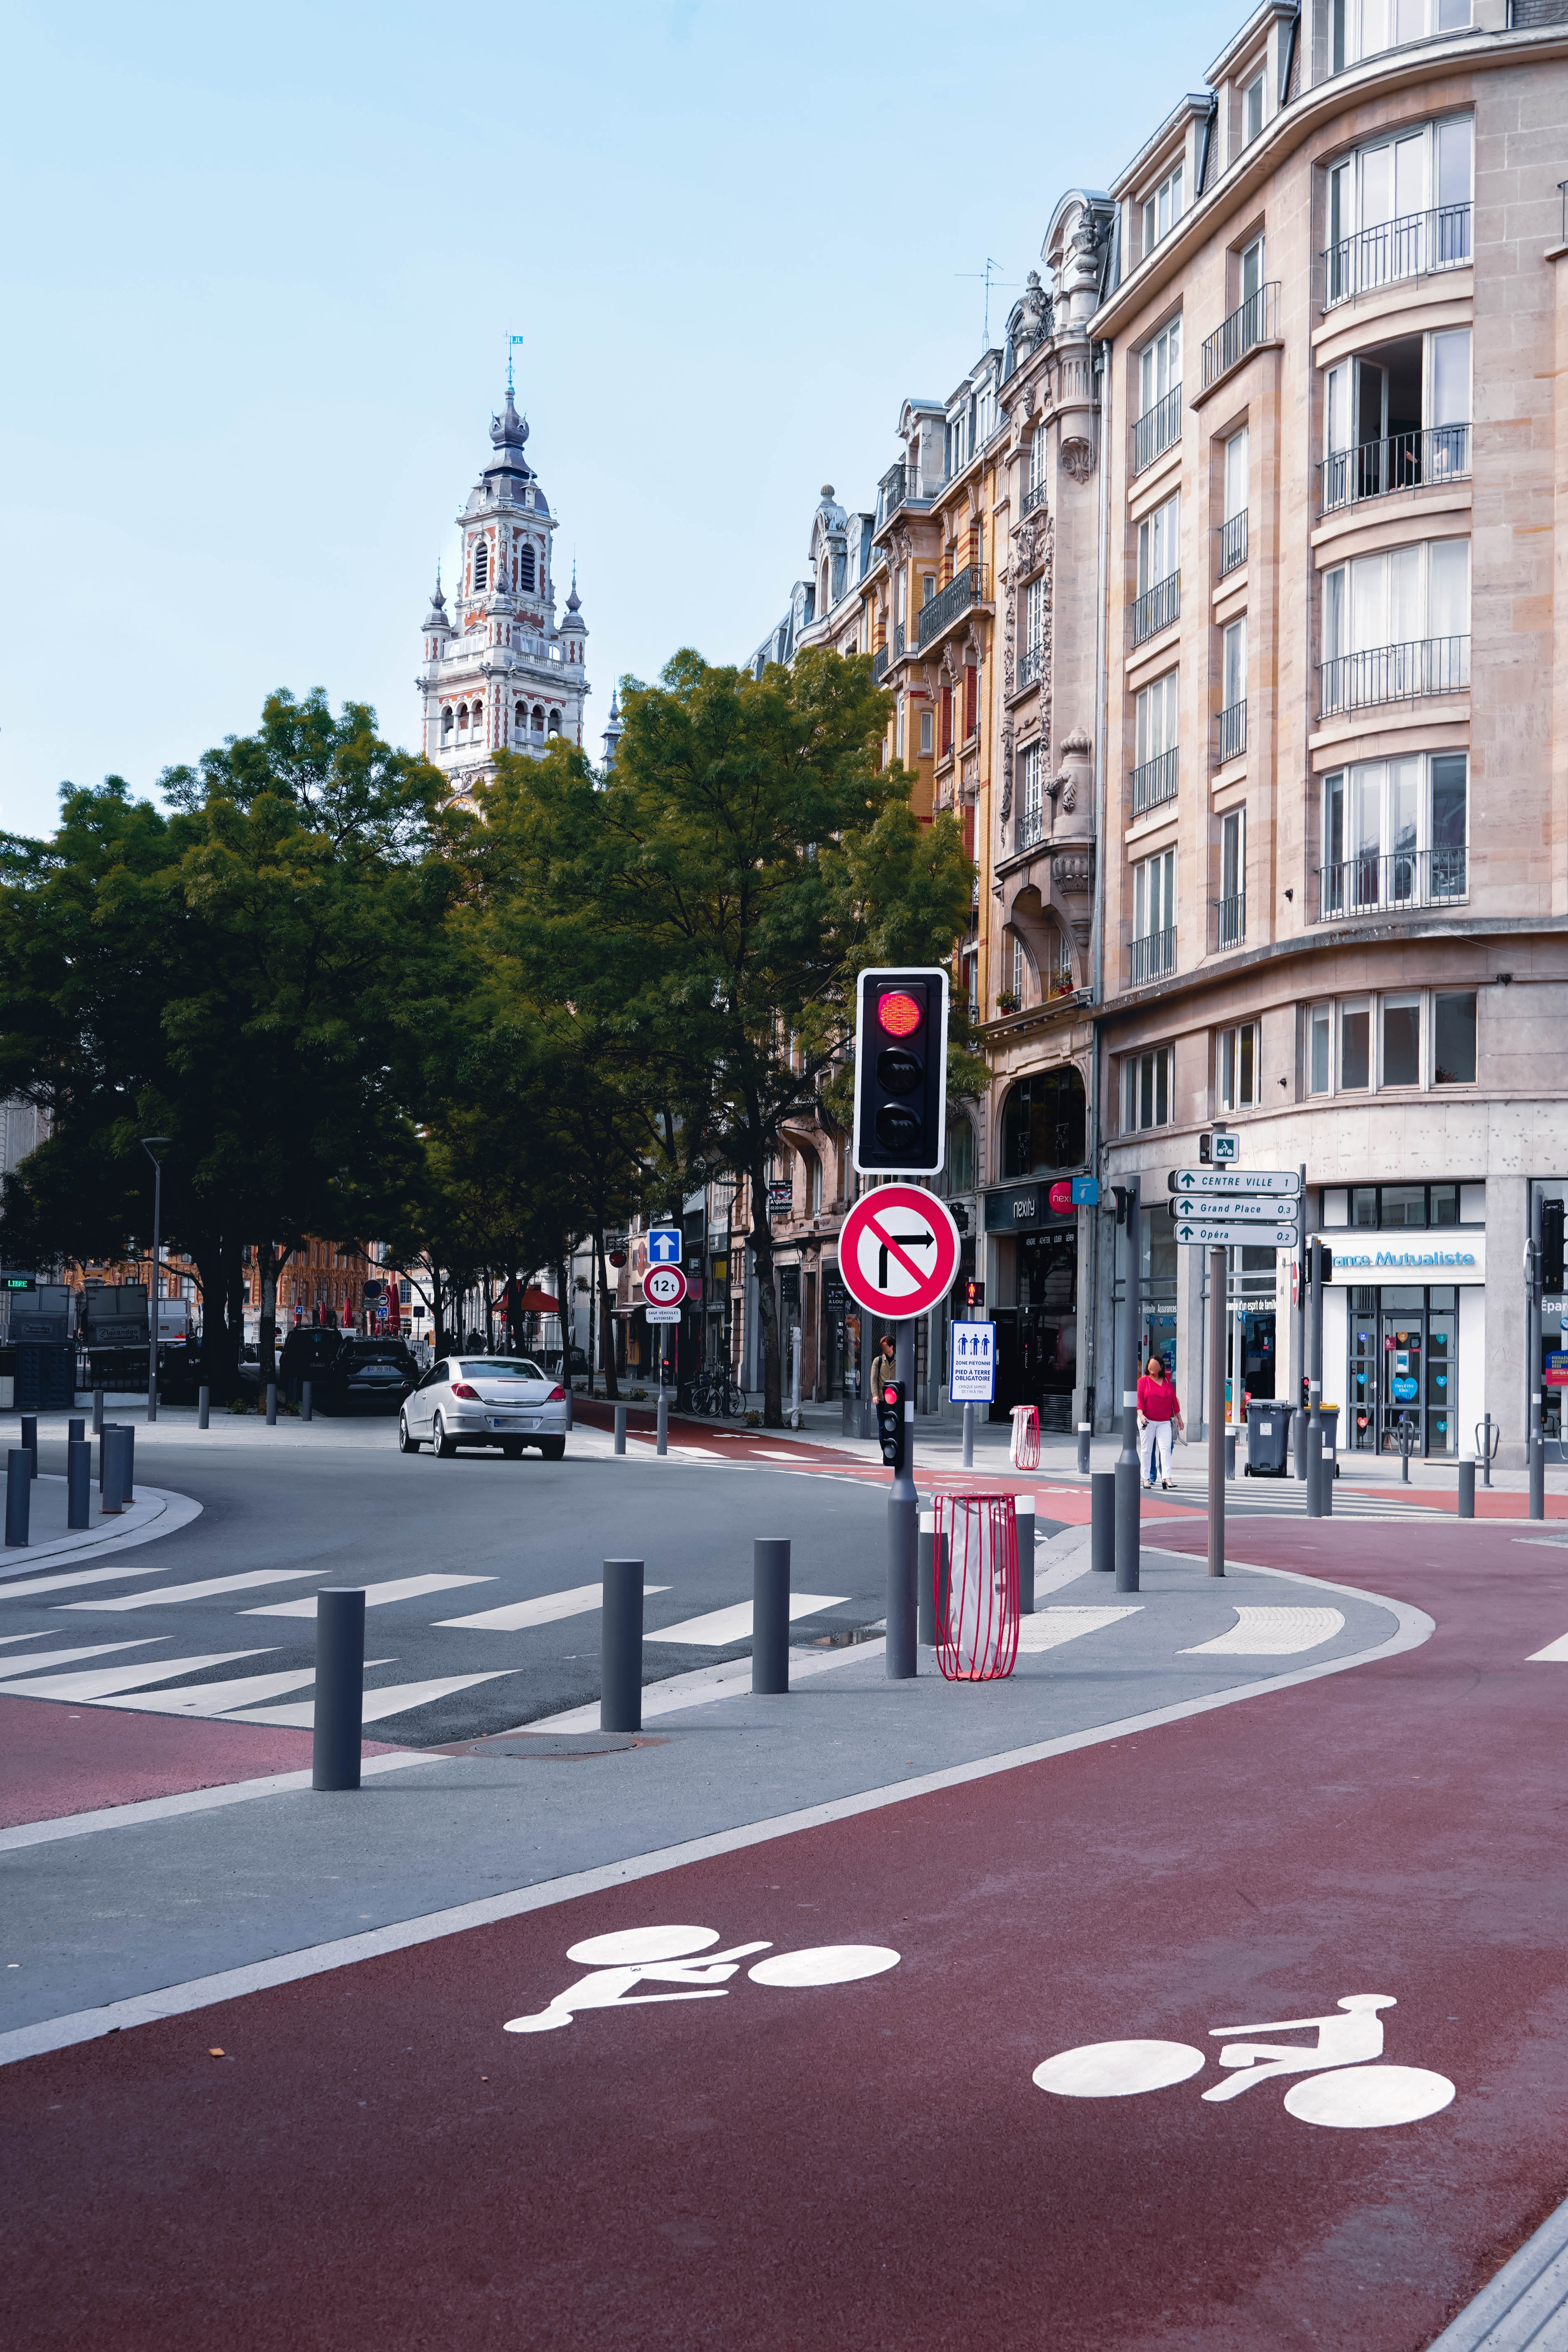
\includegraphics[width=\paperwidth,height=\paperheight]{src/Figures/Arriere_plan/Arriere_plan_Conclusion.jpg}
    }

% Rectangle
\AddToShipoutPictureBG*{
  \begin{tikzpicture}[remember picture,overlay]
    \node[fill=white, opacity=0.75, text width=\paperwidth, minimum height=5cm, anchor=north] 
    at ([yshift=-9cm]current page.north) {};
  \end{tikzpicture}
}

% Source
\AddToShipoutPictureFG*{
  \AtPageLowerRight{
    \raisebox{1cm}{
      \hspace{16cm}
      
\begin{tikzpicture}
        \node[fill=white, rounded corners=5pt, inner sep=5pt, align=center] {
          \tiny{Photography: \textcolor{blue}{Dylan Moinse (2020)}}
        };
      \end{tikzpicture}
    }
  }
}
}}

\renewcommand{\thefigure}{C.\arabic{figure}} % Numérotation spécifique pour la conclusion
\renewcommand{\thetable}{C.\arabic{table}}
\setcounter{figure}{0}
\setcounter{table}{0}

\needspace{1\baselineskip} % Reserve space
\part*{Conclusion}
    %\addcontentsline{toc}{part}{General Conclusion}
    \label{body:conclusion-generale}
    \markboth{Conclusion}{}
    \markright{Conclusion}{}
    \begin{refsegment}

    % Problem statement
\lettrine[lines=3, findent=8pt, nindent=0pt]{\lettrinefont W}{e} focused on exploring the contribution of light individual mobility to the enhancement of \acrshort{TOD}. Based on an investigation into the regional framework of station neighborhoods in the Hauts-de-France region, we have been able to assess the relevance and potential of light individual mobility in addressing the challenges of the \Commas{first and last miles} and preparing the ground for an \acrfull{M-TOD}, or transit-oriented urbanism integrating light individual mobility. Revisiting our \hyperref[introduction-generale:problematique-objectifs-hypotheses]{research problem} (page~\pageref{introduction-generale:problematique-objectifs-hypotheses}), we have sought to determine the contribution of light individual mobility in improving \gls{intermodal accessibility}, the spatial transformations induced by these redefined proximities, as well as the planning and mobility strategies aimed at promoting an \acrshort{M-TOD} model.%%Translated%%

    % Key findings
By synthesizing the main lessons learned, we have demonstrated that light individual mobility is an efficient mode of transfer in connection with exchange hubs, not only consolidating \gls{accessibility} at the local level in areas where \gls{public transport} services struggle to provide fine coverage, but also enhancing accessibility at the regional level. By expanding the influence area of station neighborhoods, light individual mobility makes intermodal travel more competitive compared to car use, especially in areas where traffic and parking conditions are restrictive. Our results also highlight that this modal complementarity cannot be fully effective without a reconfiguration of spatial structures. While some interventions are required in the immediate vicinity of public transport nodes, they are even more essential at the scale of the extended station neighborhoods, where the territorial organization often remains ill-suited for cycling practices. One of the major contributions of this thesis is the demonstration that integrating light individual mobility into the \acrshort{TOD} planning concept is not a marginal improvement, but a structural transformation of the rail-based urbanism model. This evolution calls for a rethinking of station neighborhood planning at different spatial scales, leveraging the strengths of light individual mobility to develop an urban system suited to the challenges of contemporary mobility.%%Translated%%

    % Transition hypotheses
As a critical assessment, this conclusion revisits the objectives and research hypotheses defined in the \hyperref[body:introduction-generale]{general introduction} (page~\pageref{body:introduction-generale}) and explored throughout this doctoral work. Furthermore, it aims to compare the obtained results with the expected results, presenting the key lessons learned from our research. Our approach thus involves \Commas{corroborating} or invalidating our hypotheses in light of the empirical results\footnote{
    As reported by \textcolor{blue}{\textcite[44]{tomini_methodes_2020}}\index{Tomini, Luca|pagebf}\index{Wintgens, Sophie|pagebf}, it is important to recall the \Commas{impossibility of validating hypotheses}. Indeed, a scientific hypothesis can only be refuted, but never fully validated. This epistemological stance in social sciences, or \Commas{the end of scientific certainty} \textcolor{blue}{\autocite[303]{baraquin_popper_2020}}\index{Baraquin, Noëlla|pagebf}\index{Laffitte, Jacqueline|pagebf}, is precisely the one dictated by philosophy of science teacher \textcolor{blue}{Karl~R.} \textcolor{blue}{\textcite[273]{popper_logique_1973}}\index{Popper, Karl~R.|pagebf}, according to whom a hypothesis can never be considered definitively true. It is only possible to assert that it has not yet been rejected, and thus consider it true until proven otherwise. Therefore, a hypothesis does not possess an absolute positive degree of corroboration, once it is falsified: this is the \Commas{principle of falsifiability}.
} \textcolor{blue}{\autocite[44]{tomini_methodes_2020}}\index{Tomini, Luca|pagebf}\index{Wintgens, Sophie|pagebf}, in line with the \Commas{principle of falsifiability} \textcolor{blue}{\autocite[273]{popper_logique_1973}}\index{Popper, Karl~R.|pagebf}. In this perspective, the following exercise provides a synthesis of the key contributions of the research, related to our hypotheses, which were based on a dual inductive and hypothetico-deductive approach. This approach enabled a \Commas{back-and-forth} between concepts and social realities, ensuring the richness of our geographical approach \textcolor{blue}{\autocite[24]{ageron_intermodalite-voyageurs_2013}}\index{Ageron, Pierre|pagebf}\index{Varlet, Jean|pagebf}.%%Translated%%

% --- %
    \newpage
    \needspace{2\baselineskip} % Reserve space
\section*{Summary of the Key Contributions of the Doctoral Research
    \label{conclusion-generale:principaux-apports}
    }
    \addcontentsline{toc}{section}{Summary of the Key Contributions of the Doctoral Research}
    %\markboth{Summary of the Key Contributions of the Doctoral Research}{}
    \markright{Summary of the Key Contributions of the Doctoral Research}{}

    \needspace{1\baselineskip} % Reserve space
\subsubsection*{Variations of the Planning Concept
    \label{conclusion-generale:principaux-apports-chapitre1}
    }

    % Objective 1 - Hypothesis 1 - part 1
\hyperref[objectif-1]{The first research objective} (\(O_1\), page~\pageref{objectif-1}) was to justify the relevance of an updated model that incorporates the intermodal component involving the use of individual mobility, namely an \acrshort{M-TOD}. In this regard, \hyperref[chap1:titre]{the first chapter} (page~\pageref{chap1:titre}) highlighted the contemporary issues of \acrshort{TOD}, laying the conceptual and historical foundations of this planning model (see \hyperref[table-conclusion:confrontation-hypotheses]{Table~\ref{table-conclusion:confrontation-hypotheses}} on page~\pageref{table-conclusion:confrontation-hypotheses} and \hyperref[fig-conclusion:synthese-enseignements]{Figure~\ref{fig-conclusion:synthese-enseignements}} on page~\pageref{fig-conclusion:synthese-enseignements}). In the course of this demonstration, which recounts its evolutions and adaptations, we highlighted one of the major challenges it faces today: the significant issue of the \Commas{first and last miles}. We were able to demonstrate how light individual mobility represents a strategic resource, being both more resilient and less restrictive than many innovations currently emphasized, particularly those centered around automobiles. This systemic approach to mobility thus promotes an intelligence of flows and networks, forming the core of our theoretical framework.%%Translated%%

    % Objective 1 - Hypothesis 1 - part 2
More specifically, it involves mobilizing the recent conceptualization of a \acrfull{B-TOD}. The challenge was to contextualize the recent modal diversification of \gls{bicycle} and \gls{micromobility}, which enriches this variation originally centered on conventional bicycles. We integrate a multiplicity of emerging intermodal solutions, ranging from the portability of vehicles and the rise of light electromobility, to the deployment of these vehicles in public spaces. This diversification thus extends the range of intermodal solutions, providing a more suitable and flexible response to the mobility needs expressed in different areas. As a result, we have demonstrated that, when considered separately, the two subjects of study we aim to intersect—\acrshort{TOD} and light individual mobility—are of growing interest, both in research and in planning operations (\hyperref[sous-hypothese-1.1]{\(S.H_{1.1}\)}, page~\pageref{sous-hypothese-1.1}). However, we observe that these two topics are rarely analyzed together, even though the maximization of their effectiveness relies on the strength of their interaction. It is precisely this lack of convergence that justifies the relevance of this research and the need to bridge this conceptual and operational gap (\hyperref[sous-hypothese-1.2]{\(S.H_{1.2}\)}, page~\pageref{sous-hypothese-1.2}).%%Translated%%

    % Tableau confrontation hypothèses de recherche
% Table comparing research hypotheses

    \begin{table}[h!]
    \centering
    \renewcommand{\arraystretch}{1.5}
    \resizebox{\columnwidth}{!}{
    \begin{tabular}{p{0.01\columnwidth}p{0.495\columnwidth}p{0.495\columnwidth}}
        %\hline
    \rule{0pt}{15pt} \small{\textbf{\textcolor{blue}{}}} & \small{\textbf{\textcolor{blue}{Expected Results}}} & \small{\textbf{\textcolor{blue}{Observed Results}}}\\
        \hline
\cellcolor{green!20} & \textbf{Hypothesis 1} \small{(\hyperref[hypothese-1]{\(H_{1}\)}, page~\pageref{hypothese-1})} & \cellcolor{green!20}\textbf{\small{Corroborated}}\\
\cellcolor{green!20} & \small{\textsl{The emergence of new research themes on Transit-Oriented Development and light individual mobility calls for a joint analysis.}} & \small{While these two study topics are gaining increasing interest, they are still often addressed separately, even though their synergy provides valuable insights.}\\
    \hdashline
\cellcolor{orange!20} & \textbf{Hypothesis 2} \small{(\hyperref[hypothese-2]{\(H_{2}\)}, page~\pageref{hypothese-2})} & \cellcolor{orange!20}\textbf{\small{Partially invalidated}}\\
\cellcolor{orange!20} & \small{\textsl{Research on this intermodal synergy is still conditioned by the association between bicycles and trains, and is rarely linked to the concept of urban planning.}} & \small{While \textsl{Transit-Oriented Development} is often referenced in studies, it is inadequately utilized, and the integration of new mobility solutions is becoming an increasingly important research topic, except in European contexts.}\\
    \hdashline
\cellcolor{orange!20} & \textbf{Hypothesis 3} \small{(\hyperref[hypothese-3]{\(H_{3}\)}, page~\pageref{hypothese-3})} & \cellcolor{orange!20}\textbf{\small{Partially invalidated}}\\
\cellcolor{orange!20} & \small{\textsl{The complexity of interactions between networks and territories calls for a systemic methodology capable of producing results that go beyond a simple juxtaposition.}} & \small{The complementarity of approaches has not only generated new questions but has also structured a multidimensional and multiscalar approach, albeit with risks of overlap and temporal constraints.}\\
    \hdashline
\cellcolor{green!20} & \textbf{Hypothesis 4} \small{(\hyperref[hypothese-4]{\(H_{4}\)}, page~\pageref{hypothese-4})} & \cellcolor{green!20}\textbf{\small{Corroborated}}\\
\cellcolor{green!20} & \small{\textsl{Intermodal practices, involving the use of light individual mobility, are intensifying due to the rise of micro-mobility, despite unequal adoption by certain social groups.}} & \small{Light individual mobility, as a mode of transport, is experiencing an \Commas{emergence} mainly driven by the adoption of electric scooters for personal use. However, its intermodal use is more unequal than in a monomodal context, although interventions through urban planning play a moderating role on gender inequalities.} \\
    \hdashline
\cellcolor{green!20} & \textbf{Hypothesis 5} \small{(\hyperref[hypothese-5]{\(H_{5}\)}, page~\pageref{hypothese-5})} & \cellcolor{green!20}\textbf{\small{Corroborated}}\\
\cellcolor{green!20} & \small{\textsl{With the integration of light individual mobility, multi-scalar accessibility by public transport becomes significantly more efficient, resilient, and competitive.}} & \small{Train station areas accessible by light individual mobility benefit from a local extension of their perimeter and an increase in opportunities to access regional resources. Route choices are influenced by detour and pause strategies, which, thanks to the reach and flexibility of these vehicles, optimize intermodal travel.}\\
    \hdashline
\cellcolor{green!20} & \textbf{Hypothesis 6} \small{(\hyperref[hypothese-6]{\(H_{6}\)}, page~\pageref{hypothese-6})} & \cellcolor{green!20}\textbf{\small{Corroborated}}\\
\cellcolor{green!20} & \small{\textsl{Associating light individual mobility with urban planning strategies represents an opportunity to integrate and extend train station areas, as well as to stimulate public transport usage.}} & \small{Among the main action levers for rail-oriented urban planning is the improvement of local connectivity, with a particular focus on investments in the \Commas{bike system} to boost train station usage, supporting the \acrshort{TOD} framework.}\\
        \hline
        \end{tabular}}
    \caption{Testing research hypotheses based on research conclusions.}
    \label{table-conclusion:confrontation-hypotheses}
        \vspace{5pt}
        \begin{flushright}\scriptsize{
        Author: \textcolor{blue}{Dylan Moinse (2025)}
        }\end{flushright}
        \end{table}

    \needspace{1\baselineskip} % Reserve space
\subsubsection*{Summary of Current Knowledge
    \label{conclusion-generale:principaux-apports-chapitre2}
    }

    % Objective 2 - Hypothesis 2 - part 1
\hyperref[objectif-2]{The second research objective} (\(O_2\), page~\pageref{objectif-2}) aims to critically synthesize existing knowledge and international experiences on this research topic. To this end, \hyperref[chap2:titre]{the second chapter} (page~\pageref{chap2:titre}) reviewed the current state of scientific and technical literature on \acrshort{B-TOD} and \acrshort{M-TOD}. However, while these concepts emerge implicitly in the studies analyzed, almost no research formally claims them, unlike \acrshort{TOD}, which is widely cited and used as an analytical framework (see \hyperref[table-conclusion:confrontation-hypotheses]{Table~\ref{table-conclusion:confrontation-hypotheses}} on page~\pageref{table-conclusion:confrontation-hypotheses} and \hyperref[fig-conclusion:synthese-enseignements]{Figure~\ref{fig-conclusion:synthese-enseignements}} on page~\pageref{fig-conclusion:synthese-enseignements}). The bibliometric analysis revealed a rapidly growing interest in these topics, with a doubling of the corpus over the past five years. We notably identified four major clusters of co-authors who concentrate a significant share of the bibliographic references, within Western Europe, East Asia, and the United States. The \acrfull{SLR} also identified a temporal and geographical evolution of modal combinations. Initially, research was dominated by the combination of bicycles and trains, particularly in the Old Continent, during the two decades following the formalization of \acrshort{TOD}. Then, a shift occurred towards the study of the complementarity between \acrfull{PBS} and trains. More recently, these dynamics have accelerated with the rise of \acrfull{DBS} and \acrfull{DESS}, associated with the subway. This transition is particularly visible in the other two regions of the world mentioned (\hyperref[sous-hypothese-2.1]{\(S.H_{2.1}\)}, page~\pageref{sous-hypothese-2.1}).%%Translated%%

    % Objective 2 - Hypothesis 2 - part 2
Methodologically, data collection has undergone profound transformation to adapt to the evolution of connected systems. The use of \textsl{Big Data}, combined with approaches based on advanced statistics and modeling, is gradually overshadowing traditional field survey methods. Regarding the most frequently reported results, the \acrshort{SLR} highlighted the positive influence of population and job density, as well as land-use diversity and the treatment of public spaces. These factors confirm the compatibility between the intermodal use of light individual mobility and the core principles of \acrshort{TOD}. Several shortcomings were identified following this literature review. On the one hand, there is a near absence of studies on micro-mobility and the various forms of personal-use bicycles, beyond analyses of conventional bicycles. On the other hand, there is a scarcity of studies adopting a regional scale, which is a key aspect in \acrshort{TOD} thinking. Finally, although \acrshort{TOD} is frequently mentioned, the connection between network and territory is rarely studied. The territorial approach is largely marginalized, in favor of a reading focused exclusively on transport infrastructure and services (\hyperref[sous-hypothese-2.2]{\(S.H_{2.2}\)}, page~\pageref{sous-hypothese-2.2}).%%Translated%%

    \needspace{1\baselineskip} % Reserve space
\subsubsection*{Methodological Approach
    \label{conclusion-generale:principaux-apports-chapitre3}
    }

    % Objective 3 - Hypothesis 3 - part 1
\hyperref[objectif-3]{The third research objective} (\(O_3\), page~\pageref{objectif-3}) aims to adopt a mixed methodology to address this complex topic, which encompasses a plurality of themes and territorial scales. \hyperref[chap3:titre]{The third chapter} (page~\pageref{chap3:titre}) thus provided the opportunity to define a \Commas{tailored survey}, combining quantitative and qualitative approaches adapted to a research topic that is both multidimensional and multiscalar (see \hyperref[table-conclusion:confrontation-hypotheses]{Table~\ref{table-conclusion:confrontation-hypotheses}} on page~\pageref{table-conclusion:confrontation-hypotheses} and \hyperref[fig-conclusion:synthese-enseignements]{Figure~\ref{fig-conclusion:synthese-enseignements}} on page~\pageref{fig-conclusion:synthese-enseignements}). The methodological framework relies on the integration of several complementary tools: direct observation and questionnaire surveys, \textsl{in situ} interviews, as well as the use of geostatistical analysis tools and spatial modeling. These mixed methods allowed for a progressive and structured approach, based on the different facets of the concept of \Commas{accessibility}. The goal was to produce original empirical data, enabling us to address the complexity of daily mobility and the interrelations between network and territory. First, the quantitative observation survey helped substantiate the \Commas{emergent} nature of intermodal practices involving light individual mobility at train stations. It also helped characterize the socio-demographic profile of users, cross-referencing these results with existing databases to provide a perspective on urban environmental configurations. The questionnaire survey complemented this approach by providing detailed information on mobility behaviors and motivations of cycle travelers. It also contributed to the mapping of the routes taken, offering a more refined understanding of the interrelations between intermodal practices, spaces, and locations. This approach allowed us to delve deeper into the mobility and territorial dimensions of these mobility practices, in connection with our research problem. Moreover, the use of commented journeys provided a more comprehensive perspective on users' \gls{perception} of their behaviors, accessibility conditions, and the obstacles encountered. The intention to combine methods thus enabled the integration of statistical analysis with the analysis of discourse and images.%%Translated%%

    % Objective 3 - Hypothesis 3 - part 2
Finally, thanks to the spatial modeling work, we were able to develop a more systemic analysis of the phenomena studied, integrating the determining factors identified in the \acrfull{SLR} as well as the exploratory insights derived from the field investigation. This revised model enabled us to examine the coordination of the various components of \acrshort{TOD}, laying the foundations for \acrshort{M-TOD}. As \textcolor{blue}{Hélène} \textcolor{blue}{\textcite{nessi_traduire_2022}}\index{Nessi, Hélène|pagebf} highlights, the value of this methodological combination lies not in the subordination of one approach to the other, but in their dialogue, allowing for a richer contextualization of the data and the emergence of new hypotheses (\hyperref[sous-hypothese-3.1]{\(S.H_{3.1}\)}, page~\pageref{sous-hypothese-3.1}). The application of this methodology thus allowed us to define and delimit the geographical scope of the study, based on both the railway system of the Hauts-de-France region and its \Commas{station neighborhoods}, viewed through the lens of combined walking and light individual mobility. The multiscalar strategy followed allows us to go beyond a strictly local or macro-regional reading, capturing the complexity of mobility systems and territorial dynamics. This spatial modeling and the interplay of scales were, in turn, made possible through the collection and processing of geographic data obtained from the administration of the questionnaire to cycle travelers (\hyperref[sous-hypothese-3.2]{\(S.H_{3.2}\)}, page~\pageref{sous-hypothese-3.2}).%%Translated%%

    \needspace{1\baselineskip} % Reserve space
\subsubsection*{Characterization of Mobile Individuals
    \label{conclusion-generale:principaux-apports-chapitre4}
    }

    % Objective 4 - Hypothesis 4 - part 1
\hyperref[objectif-4]{The fourth research objective} (\(O_4\), page~\pageref{objectif-4}) aims to quantify and characterize intermodal practices by focusing on the profile of users combining individual mobility and public transportation, as well as on the socio-demographic factors and resources they have at their disposal (see \hyperref[table-conclusion:confrontation-hypotheses]{Table~\ref{table-conclusion:confrontation-hypotheses}} on page~\pageref{table-conclusion:confrontation-hypotheses} and \hyperref[fig-conclusion:synthese-enseignements]{Figure~\ref{fig-conclusion:synthese-enseignements}} on page~\pageref{fig-conclusion:synthese-enseignements}). \hyperref[chap4:titre]{The fourth chapter} (page~\pageref{chap4:titre}) provided an estimate of the modal share of light individual mobility in conjunction with trains, representing around 8\% of the traveler flows observed at stations. This proportion is particularly explained by the rise of \acrfull{PeS}, which accounts for 3\%, while conventional bicycles hold a similar share. The comparative approach to modal shares reveals a growing interest in light individual mobility in peri-urban areas, provided that stations offer a minimal level of service. The hypothesis that these intermodal practices are present and expanding was confirmed: more than a third of cycle travelers, and even half of them for shared systems, \acrshort{PeS}, \acrfull{e-Bike}, and folding bicycles, report having adopted these modal combinations within the last year (\hyperref[sous-hypothese-4.1]{\(S.H_{4.1}\)}, page~\pageref{sous-hypothese-4.1}). More than half of intermodal users use these modal combinations almost daily, and three-quarters of cycle travelers are commuters. We also demonstrated a shift away from feeder buses and cars in favor of combined light individual mobility. Moreover, it appears that a significant proportion of users would completely abandon train travel if these light vehicles were unavailable. Finally, folding vehicles have a comparative advantage as they are more frequently used for both pre- and post-trip transport.%%Translated%%

    % Objective 4 - Hypothesis 4 - part 2
Based on this information about mobility behaviors, we were able to identify the characteristic traits of this social group, revealing an overrepresentation of adult men in senior managerial positions, with relatively higher levels of qualification and income. Women account for only a quarter of users, particularly regarding bicycles and \acrshort{PeS}, while half of the respondents are under 33 years old. Moreover, as age increases, gender inequalities widen, to the disadvantage of women: this reflects a dual effect of gender and age. The study thus confirmed the existence of gender inequalities in bicycle and micro-mobility use, which are even more pronounced in intermodal contexts in France. By cross-referencing these results with databases, a positive, statistically significant association was identified: between the modal share of bicycles, the level of both objective and perceived bikeability, and the proportion of female cyclists. These results demonstrate that achieving gender parity in bicycle use goes beyond considerations related to the critical mass of cyclists or the presence of cycling infrastructure. In reality, the main determinant lies in perceived bikeability. In other words, the primary focus should be on improving the \Commas{bike system} (\hyperref[sous-hypothese-4.2]{\(S.H_{4.2}\)}, page~\pageref{sous-hypothese-4.2}).%%Translated%%

    \needspace{1\baselineskip} % Reserve space
\subsubsection*{Measurement of Intermodal Accessibility Gains
    \label{conclusion-generale:principaux-apports-chapitre5}
    }

    % Objective 5 - Hypothesis 5 - part 1
\hyperref[objectif-5]{The fifth research objective} (\(O_5\), page~\pageref{objectif-5}) focuses on measuring and explaining the spatial expansion of station neighborhoods induced by light individual mobility, with the aim of assessing the intermodal accessibility gains it enables. Adopting an approach based on \Commas{effective accessibility}, which aims to diagnose the actual accessibility conditions, \hyperref[chap5:titre]{the fifth chapter} (page~\pageref{chap5:titre}) focuses on the spatiotemporal distances covered by users, in order to determine the extent to which station neighborhoods expand at the local level (see \hyperref[table-conclusion:confrontation-hypotheses]{Table~\ref{table-conclusion:confrontation-hypotheses}} on page~\pageref{table-conclusion:confrontation-hypotheses} and \hyperref[fig-conclusion:synthese-enseignements]{Figure~\ref{fig-conclusion:synthese-enseignements}} on page~\pageref{fig-conclusion:synthese-enseignements}). It also examines the factors influencing the optimization of cycling paths and the accessibility gains resulting from this optimization. The analysis established that, for commuter flows, the acceptable distance for both \gls{access} and \gls{egress} is one kilometer for combined walking and four kilometers for light individual mobility, which corresponds to an average time budget of twelve minutes. This spatial expansion results in a threefold increase in the area of station neighborhoods accessible by foot, while with light individual mobility, these neighborhoods extend up to 23 times more than traditionally accepted influence areas. At the intermodal travel scale, the median distance of a trip combining light individual mobility and trains reaches 35 kilometers, with an average duration of 53 minutes. The relevant range for this type of \gls{journey} varies according to the stages of the trip, ranging from one to four kilometers for pre-transport and one to three kilometers for post-transport. These distances, however, are modulated by the attractiveness of the stations, with those offering the best services having an effective range of five kilometers, compared to four kilometers for stations with intermediate or lower service levels.%%Translated%%

    % Objective 5 - Hypothesis 5 - part 2
The study highlights a significant improvement in accessibility rates due to the use of light individual mobility. 60\% of residents potentially have access to stations through this mode, and 70\% of the labor market becomes accessible, representing a threefold increase in the number of individuals and a twofold increase in the number of reachable jobs compared to walking combined alone. This potential is also observed in access to facilities and services, as the access potential to \acrfull{POIs} doubles, covering two-thirds of the available facilities in the region. This improvement is particularly marked for higher-category infrastructure, with 80\% becoming accessible, compared to 70\% for intermediate facilities and 60\% for local ones (\hyperref[sous-hypothese-5.1]{\(S.H_{5.1}\)}, page~\pageref{sous-hypothese-5.1}). User \gls{itinerary} choices show that travel does not always follow the most direct routes locally but includes detours, in either feeder or diffusion modes, which can be up to three times longer than the assumed path. However, this strategy helps reduce the time spent on public transport by half and decreases waiting time by 80\%. The spatiotemporal optimization of travel through \gls{detour} thus results in savings in both distance-time and spatial distance. These detours are often accompanied by better time management of the journey, integrating strategic pauses: these breaks are frequently used for daily shopping, suggesting that these trips are part of more complex mobility chains, where light individual mobility plays a central role in the link between public transport and daily activities (\hyperref[sous-hypothese-5.2]{\(S.H_{5.2}\)}, page~\pageref{sous-hypothese-5.2}).%%Translated%%

    \needspace{1\baselineskip} % Reserve space
\subsubsection*{Spatial Modeling and Action through Urban Planning
    \label{conclusion-generale:principaux-apports-chapitre6}
    }

    % Objective 6 - Hypothesis 6 - part 1
\hyperref[objectif-6]{The sixth research objective} (\(O_6\), page~\pageref{objectif-6}) focuses on identifying the key parameters to prioritize in order to effectively develop an \acrfull{M-TOD}. Unlike the previous chapters, which were based on an approach of \Commas{effective accessibility}, this final part of the doctoral research shifts to \Commas{normative accessibility}, aiming to formulate recommendations to improve accessibility while ensuring their feasibility \textcolor{blue}{\autocite[19]{levine_mobility_2019}}\index{Levine, Jonathan|pagebf}\index{Grengs, Joe|pagebf}\index{Merlin, Louis~A.|pagebf}. This prescriptive approach, however, builds on the insights drawn from \Commas{effective accessibility}, integrating the real accessibility conditions identified. \hyperref[chap6:titre]{The sixth chapter} (page~\pageref{chap6:titre}) is based on spatial modeling intended to assess the impact of various criteria contributing to the definition of a \acrshort{TOD}, incorporating an extended scope of combined walking, and an \acrshort{M-TOD} (see \hyperref[table-conclusion:confrontation-hypotheses]{Table~\ref{table-conclusion:confrontation-hypotheses}} on page~\pageref{table-conclusion:confrontation-hypotheses} and \hyperref[fig-conclusion:synthese-enseignements]{Figure~\ref{fig-conclusion:synthese-enseignements}} on page~\pageref{fig-conclusion:synthese-enseignements}). A structured analysis grid based on four key dimensions outlines the framework of the \acrfull{NPART} model: the network shape and the quality of its services (\(N\)); the degree of urban development (\(P\)); local connections and the treatment of public spaces (\(A\)); and the temporal frequency of stations, segmented by hour and period (\(RT\)). The analysis of these criteria, both from the perspective of conceptual formalization and the operationalization of \acrshort{M-TOD} principles, led to the development of recommendations for urban planning actors. It appears that the most determining criteria for station attractiveness, and thus for stimulating predicted demand, are largely related to local connectivity in station neighborhoods. More specifically, the quality of subway and tramway service plays a central role, but this dynamic is significantly reinforced by the presence of infrastructure dedicated to bicycle development, such as \acrfull{PBS} services, parking spaces, and the development of a cycling network. These elements are thus key factors in structuring \acrshort{TOD}\textcolor{blue}{s} and \acrshort{M-TOD}\textcolor{blue}{s} neighborhoods, particularly during peak hours, at both the pedestrian and cycling scales.%%Translated%%

    % Objective 6 - Hypothesis 6 - part 2
Furthermore, this overview of the key indicators defining these urban strategies also highlights a gap with the strategic directions favored by urban planners in France. Indeed, they tend to focus their efforts on access to urban centers, the commercial specialization of territories, the development of pedestrian pathways, as well as limiting motorized speed and reducing car ownership—goals that, while relevant, only partially address accessibility issues (\hyperref[sous-hypothese-6.1]{\(S.H_{6.1}\)}, page~\pageref{sous-hypothese-6.1}). The completion of the \acrshort{NPART} model led to a classification of stations and their areas of influence, identifying three distinct classes based on their potential for integration into the \acrshort{M-TOD} model. This analysis revealed that most of the stations studied have characteristics conducive to the development of an \acrshort{M-TOD} incorporating \acrshort{TOD}, but suffer from a severe lack of pedestrian and cycling connections, placing them mostly within a dynamic more closely related to \acrfull{TAD}. Thus, in the absence of genuine treatment of public spaces, these stations struggle to leverage the quality of their rail service or the concentration of human activities. One of the key insights from this advanced model is that promoting a \Commas{bike system} significantly enhances the ability of station neighborhoods to increase rail traffic. Additionally, we observed that the expansion of station neighborhoods enabled by light individual mobility results in a doubling of the number of stations meeting the criteria for an operational \acrshort{M-TOD} at the regional level, even without requiring intervention in urban forms or functions in the first instance (\hyperref[sous-hypothese-6.2]{\(S.H_{6.2}\)}, page~\pageref{sous-hypothese-6.2}).%%Translated%%

    % Figure summary of findings
    \begin{figure}[h!]\vspace*{4pt}
        \caption{Summary of Key Insights Characterizing the \textsl{Micromobility-friendly Transit-Oriented Development}}
        \label{fig-conclusion:synthese-enseignements}
        \centerline{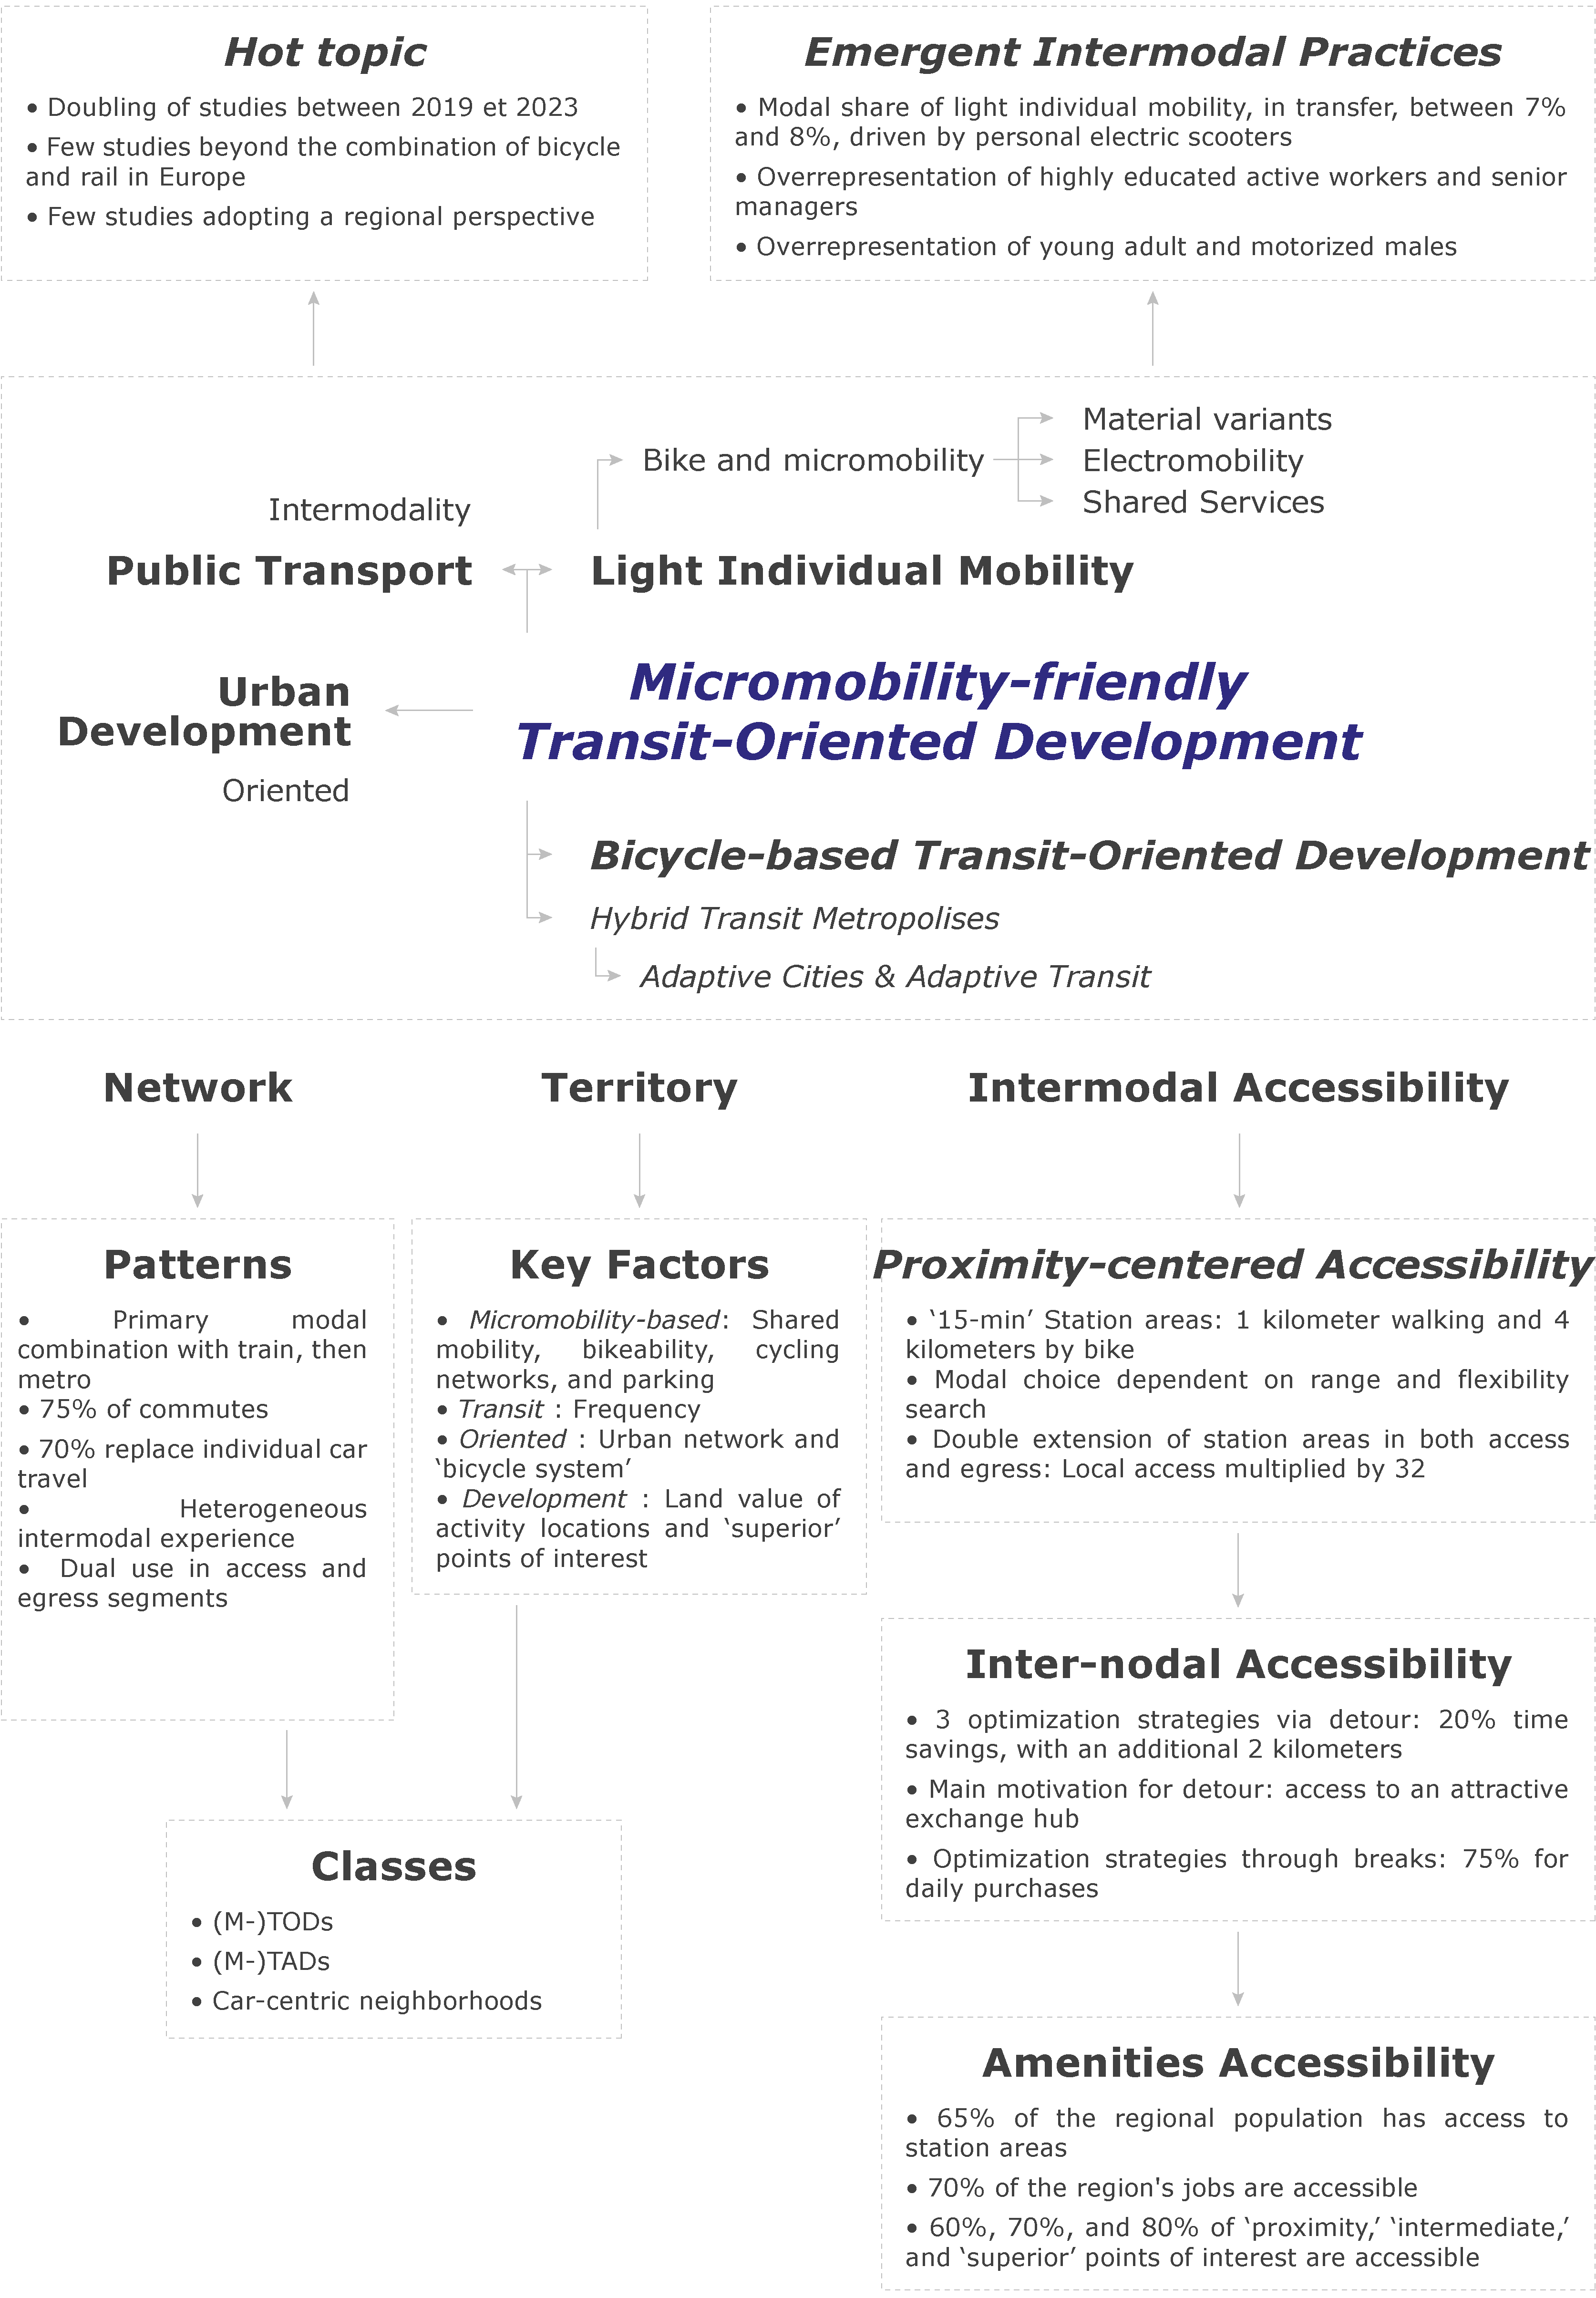
\includegraphics[width=1\columnwidth]{src/Figures/Conclusion/EN_Conclusion_generale.pdf}}
        \vspace{5pt}
        \begin{flushright}\scriptsize{
        Author~: \textcolor{blue}{Dylan Moinse (2025)}
        }\end{flushright}
    \end{figure}

    % --- %
    \needspace{2\baselineskip} % Reserve space
\section*{Reflective Scope of a \textsl{Micromobility-friendly Transit-Oriented Development}
    \label{conclusion-generale:portee-reflexive-mtod}
    }
    \addcontentsline{toc}{section}{Reflective Scope of a \textsl{Micromobility-friendly Transit-Oriented Development}}
    %\markboth{Reflective Scope of a \textsl{Micromobility-friendly Transit-Oriented Development}}{}
    \markright{Reflective Scope of a \textsl{Micromobility-friendly Transit-Oriented Development}}{}

    % Introduction
The purpose of this thesis was to demonstrate that the integration of light individual mobility into the conceptualization of an \acrfull{M-TOD} is not a mere improvement of the \acrfull{TOD}, but rather a structural transformation of the rail-oriented urbanism model. By adopting a multi-level approach, we laid the foundations for an \acrshort{M-TOD}, integrating combined walking and intermodal practices, in order to redefine the functional proximities of station neighborhoods. Theoretically, this research follows two main lines of thought: on one hand, it extends the reflections on \Commas{network urbanism} \textcolor{blue}{\autocite[]{dupuy_urbanisme_1991}}\index{Dupuy, Gabriel|pagebf}; on the other hand, it contributes to the discussions around the \Commas{mobility turn}, repositioning urban planning around renewed proximities \textcolor{blue}{\autocites{sheller_new_2006}[8]{sheller_mobilizing_2016}[13]{randell_no_2020}}\index{Sheller, Mimi|pagebf}\index{Urry, John|pagebf}\index{Randell, Richard|pagebf}. In this perspective, stations should no longer be seen as mere functional connection points, but rather as strategic intermodal spaces, located at the interface of the regional urban system. They are accessibility hubs, where light individual mobility plays a fundamental role in the network and expansion of accessible territories. These new mobility practices offer the opportunity to move beyond a segmented, mode-based, and strictly infrastructure-focused view of public transport, by improving the \Commas{relational capacity of networks} \textcolor{blue}{\autocite[15]{richer_quelles_2016}}\index{Richer, Cyprien|pagebf}\index{Meissonnier, Joël|pagebf}\index{Rabaud, Mathieu|pagebf} through a systemic \Commas{door-to-door} approach. From this point of view, \Commas{altermobility} becomes inseparable from \gls{multimodality} and intermodality \textcolor{blue}{\autocite[91-92]{vincent-geslin__2012}}\index{Vincent-Geslin, Stéphanie|pagebf}, fostering a contextualized approach to \acrshort{TOD}. A shift in reference frameworks is necessary, moving from an attractiveness logic to a territorial \Commas{hospitality} \textcolor{blue}{\autocite[2]{talandier_lhospitalite_2023}}\index{Talandier, Magali|pagebf}, which calls for a reconfiguration of urban strategies based on proximity relationships and quality of life expectations, paving the way for a new way of conceiving the interactions between urbanism and mobility.%%Translated%%

    % Accessibility
The evaluation of distance thresholds and the areas of influence associated with the routes connecting public transport stops has highlighted a joint improvement in both local and regional accessibility, resulting from intermodal practices. The integration of light individual mobility thus fosters a better connection between station neighborhoods and the rail system, while expanding access opportunities at the regional scale. Beyond the analysis of physical distances, this doctoral research aimed to incorporate one of the most comprehensive definitions of accessibility \textcolor{blue}{\autocite[3]{chapelon_accessibilite_2006}}\index{Chapelon, Laurent|pagebf}, based on four key dimensions: (i) the geographical distribution of supply and demand for resources, (ii) the performance of networks, (iii) temporality and rhythms, and (iv) the individual characteristics of users \textcolor{blue}{\autocite[128]{geurs_accessibility_2004}}\index{Geurs, Karst~T.|pagebf}\index{Wee, Bert van|pagebf}. The objective was then to evaluate how light individual mobility contributes to improving intermodal accessibility, understood both as a form of \Commas{proximity accessibility} \textcolor{blue}{\autocite[2]{silva_proximity-centred_2023}}\index{Silva, Cecília|pagebf}\index{Büttner, Benjamin|pagebf}\index{Seisenberger, Sebastian|pagebf}\index{Rauli, Anna|pagebf}; \Commas{nodal accessibility} \textcolor{blue}{\autocite[283-343]{chapelon_offre_1997}}\index{Chapelon, Laurent|pagebf}\index{Mathis, Philippe|pagebf}, as well as inter-nodal accessibility; and accessibility to resources and destinations. This paradigm shift positions accessibility not merely as a tool for facilitating travel, but as a lever for promoting proximity and reorganizing territories \textcolor{blue}{\autocite[4]{levine_century_2020}}\index{Levine, Jonathan|pagebf}. This doctoral work has shown that light individual mobility strengthens connections between places of interest at the regional scale, while promoting a return to an urban rhythm associated with \Commas{slowness} \textcolor{blue}{\autocite[9]{silva_proximity-centred_2023}}\index{Silva, Cecília|pagebf}\index{Büttner, Benjamin|pagebf}\index{Seisenberger, Sebastian|pagebf}\index{Rauli, Anna|pagebf}. In summary, the complementarity between public transport, combined walking, and light individual mobility remains largely underestimated in transport and urban planning policies. According to \textcolor{blue}{Claude} \textcolor{blue}{\textcite[6-7]{soulas_triptyque_2021}}\index{Soulas, Claude|pagebf}, an independent expert researcher, the development of combined walking and cycling can optimize public transport networks in three ways:
\begin{customitemize}
    \item First, light individual mobility helps to compensate for the heterogeneity in line load by relieving central sections while making the outer edges of networks more attractive. This reduces reliance on car park-and-ride facilities, offering viable alternatives to access exchange hubs;
    \item Second, the integration of bicycles challenges inter-station distances, which were historically calibrated to optimize local service but paradoxically contribute to reducing the commercial speed of the network;
    \item Finally, these modal synergies allow for a more linear design of public transport lines, limiting the sinuosity of routes to generating hubs, which often hampers the network's performance.
\end{customitemize}%%Translated%%

    % Cyclomobility
As the cycling infrastructure favored by cyclists, such as bike lanes, cycle tracks, and greenways, allows for longer routes by improving comfort and safety \textcolor{blue}{\autocite{poisson_amenagements_2019}}\index{Poisson, Adrien|pagebf}\index{Chapelon, Laurent|pagebf}\index{Lammoglia, Adrien|pagebf}, the development of an urban system combined with a \Commas{bike system} strategically oriented towards public transport networks stands out as a key leverage point to reconcile sustainable proximity travel and connections with exchange hubs. More generally, this reflection leads us to consider \Commas{cyclomobility}, a concept analogous to \Commas{automobility}, which distinguishes three interacting dimensions \textcolor{blue}{\autocite[20-21]{rerat_au_2019}}\index{Rérat, Patrick|pagebf}: \textsl{usage}, which refers to socio-demographic characteristics and travel patterns; \textsl{cycling mobility potential}, which refers to access to bicycles, skills, motivations, and social representations; and \textsl{territorial reception potential}, which refers to the bikeability of territories as well as their norms and policies. According to \textcolor{blue}{Matt} \textcolor{blue}{\textcite[492]{watson_how_2012}}\index{Watson, Matt|pagebf}, researcher and professor at the University of Sheffield, \Commas{cyclomobility} and \Commas{automobility} systems are in direct competition for access to the same resources, both material and symbolic. In other words, the development of a structured and connected cycling network requires a reconfiguration of urban infrastructures, often marked by a hierarchy that favors motorized vehicles. This phenomenon is notably illustrated in station neighborhoods, where the massive presence of automobile infrastructure acts as a barrier to the growth of cycling as a feeder mode to public transport hubs. Ultimately, the relatively low proportion of intermodal travel observed today should not overshadow its strong development potential, particularly due to the capacity of light individual mobility to capture the modal shift from car users in peri-urban areas \textcolor{blue}{\autocite[22]{ulles_quelle_2024}}\index{Ullès, Jean-Clément|pagebf}\index{Chapelon, Laurent|pagebf}. Even though a \Commas{culture of indifference towards public transport} persists and continues to prevail \textcolor{blue}{\autocite[656]{tan_identifying_2014}}\index{Tan, Wendy|pagebf}\index{Bertolini, Luca|pagebf}\index{Janssen-Jansen, Leonie|pagebf} in these urban contexts, creating an obstacle to an integrated mobility vision, the operationalization of \acrshort{M-TOD} relies on concrete levers of action, which must be activated by urban planning and transport actors to accelerate the transition towards a rail-based urbanism capable of addressing current regional challenges.%%Translated%%

    % --- %
    \needspace{1\baselineskip} % Reserve space
\section*{Implications of the Doctoral Research
    \label{conclusion-generale:implications}
    }
    \addcontentsline{toc}{section}{Implications of the Doctoral Research}
    %\markboth{Implications of the Doctoral Research}{}
    \markright{Implications of the Doctoral Research}{}

    % Introduction
Building on the insights gained, we aimed to formulate various recommendations for urban planning actors, in support of public policies on urban development and transport. These recommendations are not intended to be exhaustive, nor to propose a level of detail that would allow for their immediate integration into strategic directions. Rather, they resemble guiding principles, akin to a manifesto, designed to inspire new approaches and methods and provide avenues for reflection that can be adapted to different contexts. These recommendations, presented in sections, are part of a logic of activating transition levers, offering strategic action lines to promote the integration of light individual mobility into station neighborhoods and strengthen intermodality within public transport networks. The directions we suggest are divided into ten distinct sections, incorporating a range of possible measures and initiatives, detailed below.%%Translated%%

    \needspace{1\baselineskip} % Reserve space
\subsubsection*{Strategic and Organizational Avenues
    \label{conclusion-generale:implications-gouvernance}
    }

    % Urban Planning Documents
    \begin{displayquote}
\textbf{Section 1: Positioning Station Neighborhoods as Strategic Areas at the Heart of Territorial Development Strategic Directions.}
\\
\textsl{Integrate and reassess the functional boundaries of station neighborhoods in strategic urban and mobility planning frameworks.}
    \end{displayquote}
The goal of the first section of the recommendations is to redefine the extended boundaries of station neighborhoods within urban and mobility planning documents, in order to go beyond the limitations of planning that focuses exclusively on the immediate proximity of exchange hubs. Currently, most urban and transport strategies continue to consider station neighborhoods within narrow boundaries, often defined at the scale of traditional pedestrian accessibility, thus overlooking the potential for extension afforded by the enhancement of \gls{walkability} and bikeability. This approach calls for a revision of urban planning documents and mobility plans—such as \acrfull{SCoT}, \acrfull{PLU}, and \acrfull{PDM}—to adapt regulatory and operational frameworks to extended station neighborhoods. By using the measurement and mapping tools developed in this research, it becomes possible to rethink zoning around exchange hubs, taking into account the actual areas of influence of stations.%%Translated%%

    % Observatory
    \begin{displayquote}
\textbf{Section 2: Transform Station Neighborhoods into Laboratories for Urban Innovation and New Planning Practices.}
\\
\textsl{Establish an observatory focused on transit-oriented urban planning and intermodality, aimed at evaluating initiatives and experiments.}
    \end{displayquote}
The goal of the second section is to develop dedicated bodies for studying the interactions between urbanism and mobility, with an intermodal focus, thereby positioning station neighborhoods within a dynamic of experimentation and continuous evaluation. From the perspective of diffusion and transferability of \Commas{best practices}, these observatories would serve as analytical tools to measure the evolution of intermodal practices, assess experiments related to feeder systems and urban frameworks, and adapt public policy support based on empirical results. Beyond their role in monitoring, evaluation, and comparison between territories, these systems would provide a structured methodological framework for testing and comparing different configurations for integrating light individual mobility into exchange hubs, through pilot zone experiments while collecting useful data. They would thus contribute to a better understanding of the factors influencing the adoption of intermodal practices and help anticipate emerging trends in mobility and the planning of rail-based territories. The operationalization of such a transversal structure would require close collaboration between local authorities, transport operators, researchers, associations, and the users themselves, for informed decision-making.%%Translated%%

    \needspace{1\baselineskip} % Reserve space
\subsubsection*{Action Lines to Promote Intermodality
    \label{conclusion-generale:implications-mobilites}
    }

    % Passenger Information
    \begin{displayquote}
\textbf{Section 3: Deploy Tools for Information and Communication Dedicated to Intermodality.}
\\
\textsl{Improve access to information and raise awareness of the benefits of intermodal use of light individual mobility.}
    \end{displayquote}
The third section of the recommendations focuses on improving information, communication, and awareness regarding intermodal journeys involving light individual mobility. We recommend developing algorithms coupled with dynamic maps, accessible both physically in stations and public spaces, and digitally through mobile apps and online platforms. These interactive tools would allow potential users to identify in real time the infrastructures and services facilitating intermodality, such as secure cycling routes, bike parking spaces, sharing services, and intermodal connections that can be optimized. By integrating multimodal navigation features, similar to \acrshort{MaaS}, these applications would offer optimized route suggestions, taking into account user preferences and the availability of rental and secure parking services. At the same time, a targeted communication strategy, as well as the use of \Commas{gamification}, would encourage the adoption of these intermodal practices by highlighting the benefits of light individual mobility in the context of feeder systems to stations. Awareness campaigns, in the form of local actions, promotional events, and partnerships with transport and planning actors, would help remove the cognitive and cultural barriers associated with these new practices. The goal would be to create an environment conducive to intermodality, where accessibility to information and the promotion of alternatives to individual car use play a key role in changing behaviors.%%Translated%%

    % Shared Mobility
    \begin{displayquote}
\textbf{Section 4: Develop a Network of Shared Mobility Services at the National or Regional Scale, with a Strategic Grid of Exchange Hubs and Station Neighborhoods.}
\\
\textsl{Strengthen intermodality by developing a national or regional network of shared mobility services within the influence areas of exchange hubs.}
    \end{displayquote}
The fourth section of the recommendations aligns with a logic of modal complementarity and enhances the visibility of light individual mobility in urban spaces. It proposes developing a network of bike and/or scooter-sharing services, deployed strategically around exchange hubs to facilitate intermodality and extend the possibilities for feeder systems to stations. The main goal is to integrate both short- and long-term rental services, accessible for both occasional and daily use. This involves developing a fleet of shared vehicles, electric or non-electric, operated by an entity at a relevant geographic scale aligned with the intermodal system\footnote{
    Implementing such a mobility service, by a public or private operator, inevitably raises the question of the associated business model, which remains to be defined.
}, i.e., at the regional or national level, similar to the Dutch or Belgian experiences, rather than within segmented metropolitan or municipal boundaries. The success of such a system depends on establishing a dense network of drop-off stations, located not only at and around stations but also within extended station neighborhoods, where feeder needs are most significant. To optimize the use of these services and enhance their attractiveness, it is essential to support this deployment with integrated ticketing, allowing access to both public transport systems and shared mobility services through a single ticket. This unified ticketing could be coupled with financial incentives, such as offering discounts to public transport subscribers. In this regard, this direction resonates with the regional ambitions outlined in Principle 18 of the Vélo Plan, part of the \acrfull{SRADDET} of the \textcolor{blue}{\textcite[40]{region_hauts-de-france_plan_2023}}\index{Région Hauts-de-France@\textsl{Région Hauts-de-France}|pagebf}. This suggestion explicitly mentions the intention to launch a \Commas{\textsl{bike-sharing experiment at the scale of a territory or a train line.}} The report issued by the \textcolor{blue}{\textcite[75]{ceser_hauts-de-france_mobilite_2021}}\index{CESER Hauts-de-France@\textsl{CESER Hauts-de-France}|pagebf}\index{Bally, Stéphane|pagebf}\index{Melcus, Alain|pagebf} also supports this direction, even though this body emphasizes the interest in a regional-scale rental system rather than patchwork services.%%Translated%%

    % Boarding Policy
    \begin{displayquote}
\textbf{Section 5: Implement a Bicycle and Scooter Boarding Policy Focused on Express Rail Services, Integrating Dedicated Spaces to Facilitate the Boarding of the Most Compact Vehicles.}
\\
\textsl{Promote intermodality by facilitating the boarding of bicycles and micro-mobility devices on express rail services.}
    \end{displayquote}
The fifth section focuses on the evolution of bicycle and micro-mobility boarding policies on trains\footnote{
    The hospitality of territories also involves better accommodation of light individual mobility in public transport, but perhaps also a form of reciprocity between these vehicles and the infrastructures that host them. Some incidents illustrate the challenges of this coexistence. For example, in 2022, a \acrfull{PeS} caught fire aboard a train in Spain, leading regulatory authorities to ban their boarding a year later \textcolor{blue}{\autocite{cottrel_trottinette_2022}}\index{Cottrel, Olivier|pagebf}. This incident raises safety concerns, particularly regarding the quality of electric batteries. In this sense, this factual element highlights how essential it is to involve both regulatory efforts on one hand and technical and usage improvements on the other.
}, with the aim of facilitating intermodal travel. In line with our observations and with a focus on optimizing flows, it would be pertinent to prioritize express trains over omnibus-type rail services for the development of dedicated compartments for these vehicles. These trains, due to their longer distances and limited number of stops, are particularly strategic for fostering intermodal travel across expanded territories, where the combination of train and light individual mobility offers a credible alternative to car use. Special attention should be given to compact and easily transportable vehicles, such as folding bikes and \acrfull{PeS}, which currently lack any suitable facilities in most trains. Yet, these vehicles are particularly suited to intermodal practices. The integration of specific spaces for these devices would therefore improve the comfort and fluidity of intermodal travel, while enhancing their competitiveness against exclusive car use. In this regard, the development of modular compartments, tailored to the type of vehicle within the train cars, would represent an interesting innovation.%%Translated%%

    % Parking Policy
    \begin{displayquote}
\textbf{Section 6: Strengthen the Provision of Secure Parking Near Exchange Hubs and in Station Neighborhoods, Ensuring Attractive Capacity and Access, as Well as Adaptation to the Type of Vehicle.}
\\
\textsl{Develop secure, accessible parking infrastructure within extended station neighborhoods, adapted to the diversification of light individual mobility.}
    \end{displayquote}
The sixth section of the recommendations focuses on the development of parking infrastructure adapted to bicycles, in order to facilitate the intermodal adoption of light individual mobility and enhance the attractiveness of public transport networks. One of the main barriers to combined bike and train use is the lack of secure, adapted spaces for parking vehicles. To address this challenge, it is necessary to install secure parking infrastructure not only in the immediate vicinity of stations but also within extended station neighborhoods, where feeder needs are particularly high. These spaces should be designed to accommodate a variety of vehicles. These infrastructures could also include charging stations for electric or assisted mobility modes. Similarly, the implementation of secure lockers for compact vehicles would provide a complementary solution to encourage their use in intermodal travel. While large metropolitan stations are seeing the emergence of capacity bike stations, driven by the \acrfull{LOM}, secondary stations could benefit from shared parking spaces or individual lockers. The accessibility of these parking facilities must be designed to facilitate their daily use, either by ensuring open, free access in the \gls{public space} or by ensuring interoperability with public transport systems. An integrated access principle, via a transport ticket or subscription, would ensure continuity of service and enhance the attractiveness of the intermodal system. The implementation of flow tracking sensors would allow the infrastructure to adapt to needs by anticipating necessary expansions.%%Translated%%

    \needspace{1\baselineskip} % Reserve space
\subsubsection*{Improvement Avenues for Designing Station Neighborhoods
    \label{conclusion-generale:implications-amenagement}
    }

    % Cycling Infrastructure
    \begin{displayquote}
\textbf{Section 7: Strengthen the Connectivity of Station Neighborhoods through a Structuring, High-Quality, and Secure Cycling Network.}
\\
\textsl{Structure an intermunicipal cycling network to extend and improve access to stations.}
    \end{displayquote}
Developing an intermunicipal network of continuous and secure cycling routes, linking extended station neighborhoods to railway stations and also connecting station neighborhoods to each other, represents the seventh section. This objective translates into strengthening cycling connectivity by ensuring direct, secure, and comfortable infrastructure, while addressing urban cutoffs. In the same spirit, priority should be given to pedestrian and cycling continuities, particularly along major structural routes \textsl{within} and \textsl{between} station neighborhoods, in order to create connections between stations, thus enhancing the permeability of the public transport network. The goal is to ensure an effective feeder system, initially based on major routes connected to transport hubs, on intersections, and structuring secondary roads. To structure and prioritize this cycling network, aligning routes as \Commas{bike highways} or a unifying \Commas{\acrshort{RER} bike} project would represent a major advancement. These strategic cycling networks would allow for the identification of the most essential corridors and promote integrated planning of the cycling network at the regional scale. This initiative should also be accompanied by work on visual identity and signage, to make the network more identifiable and attractive to cycle travelers and cyclists. The installation of clear and uniform signage, combined with dedicated services such as rest areas, repair stations, and electric charging stations, would help make these routes more accessible and functional. These recommendations align with the strategic orientation recommendations already formulated at the regional level. The report by the \textcolor{blue}{\textcite[72]{ceser_hauts-de-france_mobilite_2021}}\index{CESER Hauts-de-France@\textsl{CESER Hauts-de-France}|pagebf}\index{Bally, Stéphane|pagebf}\index{Melcus, Alain|pagebf}, focusing on regional territorial development, recommends building an intermunicipal cycling network, with one of its main objectives being to facilitate access to stations in addition to bike rental and parking infrastructure.%%Translated%%

    % Restricting the Car
    \begin{displayquote}
\textbf{Section 8: Reduce the Presence of the Car in Station Neighborhoods.}
\\
\textsl{Rebalance the allocation of public space by limiting car usage in station neighborhoods.}
    \end{displayquote}
The eighth section of the recommendations follows a coercive approach to land use planning, based on the results of this research regarding the competitiveness of intermodality in relation to the car. Our analysis shows that intermodality only becomes truly competitive when the urban environment imposes constraints on individual car use. The goal is to act on several levers simultaneously to limit \Commas{car dependence}. The first measure concerns reducing car traffic by addressing traffic flow and speed within the station areas. By establishing calm zones where traffic is restricted or limited to lower speeds, it becomes possible to rebalance public space in favor of walking and cycling. This initiative should be accompanied by pedestrianization of certain major roads, creating comfortable routes to stations. In addition, the gradual reduction of car parking spaces within station neighborhoods represents a strategic lever to discourage the habitual use of private cars. This does not mean eliminating these facilities, but rather adapting their number and management, to prioritize alternative solutions such as park-and-ride facilities, shared spaces, or carpooling areas. In parallel, introducing disincentive parking pricing measures could be an effective tool for influencing modal choices. The implementation of differentiated pricing, based on parking duration or personal circumstances, would encourage drivers to prioritize other modes of transport.%%Translated%%

    \needspace{1\baselineskip} % Reserve space
\subsubsection*{Proposals for Integrated Planning at the Regional Scale
    \label{conclusion-generale:implications-planification}
    }

    % Urbanism
    \begin{displayquote}
\textbf{Section 9: Intervene on Activities and Built Forms to Increase Density and Diversify Uses.}
\\
\textsl{Adapt urban forms and activities for a \Commas{Quarter-Hour} Urbanism.}
    \end{displayquote}
This ninth section involves measures to densify and diversify urban activities in order to reconfigure urban forms, urban rhythms, and proximities within station neighborhoods. One of the goals is to concentrate and more effectively distribute residential, commercial, and other functions around exchange hubs, in order to promote more balanced urbanization and intensify uses near stations. This is not only about increasing built density but, more importantly, about fostering a diversity of urban functions that ensures a better distribution of flows. The central challenge of this section is thus to rethink the urban fabric of station neighborhoods through the lens of the \Commas{Quarter-Hour} principle. The idea is to adopt an approach that allows each resident or user to access key urban amenities within fifteen minutes, whether by foot, by bike, or by public transport. Such a redesign involves revising urban planning regulations and territorial planning tools to encourage the construction of housing near stations, while ensuring a balanced distribution of housing types. Ultimately, this ninth section calls for a profound and systemic transformation of urban and transport policies, placing proximity, accessibility, and intermodality at the heart of planning strategies.%%Translated%%

    % Artificialization
    \begin{displayquote}
\textbf{Section 10: Regulate Land Artificialization to Preserve Land Resources.}
\\
\textsl{Implement a systemic land-use sobriety policy in connection with the \acrshort{M-TOD}.}
    \end{displayquote}
Limiting land artificialization is a major long-term challenge, as demonstrated by this tenth section of the recommendations. The goal is to avoid excessive urban sprawl and preserve natural and agricultural areas located on the outskirts of station neighborhoods, while ensuring controlled and sustainable urbanization. In this perspective, the urbanization of railway zones should be primarily focused on already artificialized spaces, by promoting the rehabilitation of brownfields and the densification of built-up areas rather than uncontrolled urban expansion. The challenge is thus to reconcile urban growth with land-use sobriety, in line with recent public policies aimed at slowing down and compensating for urbanization, stemming from the \acrfull{ZAN} goal. Long-term urban strategies thus involve the issue of land control, which can be addressed through the creation of green and blue networks coordinated with the urban development model. This approach aims to enhance quality of life by reducing urban heat islands and improving the landscape. The presence of vegetation, bodies of water, and recreational spaces near public transport infrastructure supports the social acceptability of development projects, while playing a key role in improving the attractiveness of public transport networks and quality of life. Ultimately, this tenth section calls for resilient and ecological urban planning, combining controlled densification and \Commas{building the city on the city}.%%Translated%%

    % --- %
    \needspace{1\baselineskip} % Reserve space
\section*{Extensions and Research Perspectives
    \label{conclusion-generale:perspectives}
    }
    \addcontentsline{toc}{section}{Research Perspectives}
    %\markboth{Research Perspectives}{}
    \markright{Research Perspectives}{}

% Introduction
While this research has provided conceptual, methodological, and empirical contributions to this research topic, certain inherent limitations of the approach and the study areas must be acknowledged. Indeed, all research is conducted within a constrained methodological and temporal framework, which guides the analysis and conditions the results obtained. This final section thus aims to clarify the limitations of this work, from the perspective of the data used, the methods employed, and the scope of the conclusions, while proposing future research avenues that could extend and deepen these reflections. In light of these limitations, this reflection on the possible boundaries and extensions allows for the identification of complementary areas of investigation that could be explored by both academic research and operational stakeholders, in order to refine, improve, and adapt the \acrshort{M-TOD} model to different contexts.%%Translated%%

    \needspace{1\baselineskip} % Reserve space
\subsubsection*{Conceptual Deepening
    \label{conclusion-generale:perspectives-pistes-theoriques}
    }

 % Proximity
Conceptually, the integration of light individual mobility within the \acrshort{M-TOD} leads to a re-examination of the notion of proximity, linking it with other emerging trends in urbanism and spatial planning. While the renewed concept of the \Commas{15-Minute City} has been widely used in this research, it is due to its proven complementarity with \acrshort{TOD} and \acrshort{M-TOD}, a relationship now recognized within a broad scientific community. In this regard, several recent approaches have contributed to refining this connection, particularly through \textsl{Transit-Oriented Development-based 15-minute cities}, which highlight the compatibility and synergies between these two urban development models \textcolor{blue}{\autocite[11]{wolanski_potential_2023}}\index{Wolański, Michał|pagebf}. These reflections are part of a broader approach centered on user experience and urban quality, similar to \textsl{People-Oriented Development}, which aims to place social and territorial dimensions at the heart of urban and transport strategies. This concept thus contributes to a wider reflection on proximities and the interactions between infrastructure and mobility practices, and represents a fruitful avenue for renewing the approach to urban planning \textcolor{blue}{\autocite{davis_people_2024}}\index{Davis, Michael Maks|pagebf}\index{Verlinghieri, Ersilia|pagebf}. Finally, a more recent evolution in the academic debate deserves mention: \textsl{Proximity-Oriented Development}, which seeks to bring \acrshort{TOD} into dialogue with territorial proximities and geoproximities. This involves deepening the concept of proximity, not only as a simple territorial resource but by linking it with \Commas{proxibility}, understood as a territorial asset \textcolor{blue}{\autocite{lebrun_proximite_2024}}\index{Lebrun, Nicolas|pagebf}. Although still in the process of formalization, this conceptual framework offers an exciting perspective for this doctoral research, extending the reflection on the integration of light individual mobility \textcolor{blue}{\autocite[3]{plastara_15-minute_2023}}\index{Plastara, Dimitra|pagebf}\index{Pozoukidou, Georgia|pagebf}.%%Translated%%

% Cycles as a Network
From a more practical perspective, it seems valuable to further explore the close relationship between the public transport network and the cycling network, by considering the notion of \Commas{bike system} as an integral component of a structuring transport network. This perspective is fully aligned with current urban development dynamics, particularly through the \Commas{\acrshort{RER} bike} initiatives, which take the principles of regional railway network structuring and propose \Commas{bike highways}, characterized by identifiable routes and stops marking points of interest, equipped with amenities and services. By thus materializing a systemic organization of cycling flows, these infrastructures go beyond the simple conception of the bike as an individual mode of transport, making it a vector of territorial mobility, capable of structuring daily travel at the metropolitan and regional scales. Consequently, an exciting research avenue would be to analyze the \Commas{bike system} as a full-fledged public transport network, questioning how it meets similar network structuring, performance, and interconnection logics. Just as there is a \Commas{natural} connection between an interurban railway network and an urban railway network—such as the connection between \acrshort{TER} and the subway—it would be interesting to explore the relationships between cycling network nodes and railway stations, within an integrated vision of mobility.%%Translated%%

    \needspace{1\baselineskip} % Reserve space
\subsubsection*{Avenues for Methods and Analytical Tools
    \label{conclusion-generale:perspectives-pistes-methodes}
    }

% Quantitative - Limitations
Considering the methodology, the approach adopted has certain limitations, particularly with regard to the use of quantitative approaches: the representativeness of the samples and the extrapolation of results are two representative factors. The sample of cycle commuters studied, based on quantitative observation and the questionnaire, could be expanded to better integrate underrepresented populations and account for the specificities of each type of vehicle within light individual mobility. Another methodological bias lies in the focus on the actual use of the observed modal combinations, to the detriment of an analysis of the \Commas{non-use} phenomenon, that is, individuals who have not adopted these practices but exhibit potential for modal shift. This limitation concerns not only \Commas{non-cyclists}, but also \Commas{new cyclists}, as well as \Commas{misuse} practices, which would deserve further investigation. Finally, the difficulty in evaluating the long-term impact of integrating light individual mobility into \acrshort{TOD} strategies \textcolor{blue}{\autocite{}} constitutes another weakness of the doctoral research. This is because it relies primarily on static data, captured at a specific moment in time, whereas a longitudinal approach would allow for a better understanding of the evolution of intermodal practices and the transformation of station neighborhoods over a more extended period.%%Translated%%

% Quantitative - Avenues
To address these methodological limitations, several avenues for improvement can be considered. First, a more systematic approach to the processing of big data would help compensate for sampling biases and refine the analysis of intermodal behaviors. The use of data from \textsl{Big Data}, including ridership data provided by transport operators and GPS tracks extracted from smartphones, would offer a more nuanced and dynamic view of flows carried out with \acrshort{PBS} services, \acrshort{DBS}, \acrshort{DESS}, as well as with bicycles or personal mobility devices. Regarding analytical tools, the challenge would be to develop prospective scenarios, supported by multi-agent modeling, now feasible thanks to the initial insights gathered on \Commas{typical} user behaviors. Adopting a \Commas{microscopic} approach, using advanced tools such as the open-source project \acrfull{MATSim}, would allow for the simulation of individual mobility behaviors, taking into account the specific characteristics of travelers and various prospective scenarios, while reintegrating these behaviors within the framework of their allocation to the transport network \textcolor{blue}{\autocite[119]{chapelon_transports_2016}}\index{Chapelon, Laurent|pagebf}. Such an approach would have the advantage of better understanding the population of \Commas{non-cyclists}, which is often marginalized in current studies \textcolor{blue}{\autocite{poisson_amenagements_2019}}\index{Poisson, Adrien|pagebf}\index{Chapelon, Laurent|pagebf}\index{Lammoglia, Adrien|pagebf}.%%Translated%%

% Qualitative - Limitations
In the spirit of a \Commas{microscopic} scale of analysis with a more qualitative perspective, the \Commas{macro-spatial} approach adopted in this thesis, based on the interaction between network and territory at the regional scale, involves certain limitations in terms of considering socio-spatial dynamics at finer scales. Indeed, this research does not claim to encompass all the explanatory factors of mobility practices, particularly concerning the \Commas{meso-} and \Commas{micro-spatial} scales, where more subtle adjustments in usage and modal strategies occur \textcolor{blue}{\autocite[7]{desjeux_sciences_2004}}\index{Desjeux, Dominique|pagebf}. Certainly, the exploratory realization of commented journeys constitutes a first \Commas{nano-sociological} approach, integrating the normative, unconscious, and affective dimensions of mobility behaviors \textcolor{blue}{\autocite[7]{desjeux_sciences_2004}}\index{Desjeux, Dominique|pagebf}. However, these qualitative surveys, while essential, are limited in number and would benefit from being expanded and diversified in order to encompass a variety of contexts and user profiles. Furthermore, while the focus on urban dimensions in this research is indispensable for understanding the spatial configurations of intermodal mobility, it cannot, by itself, explain all the social dynamics that shape intermodal practices \textcolor{blue}{\autocite[4]{gaudron-arlon_gender_2022}}\index{Gaudron-Arlon, Léa|pagebf}. It therefore appears essential to adopt a multidimensional approach, combining spatial, social, and individual challenges, in order to capture the complexity of travel chains \textcolor{blue}{\autocite[7]{heesch_gender_2012}}\index{Heesch, Kristiann~C.|pagebf}\index{Sahlqvist, Shannon|pagebf}\index{Garrard, Jan|pagebf}.%%Translated%%

% Qualitative - Avenues
To deepen these qualitative dimensions, several research avenues can be considered. One of them would involve using the concept of \Commas{motility}, conceived as a mobility capital, which reflects the articulation between mobility opportunities, individual resources, and individuals' social predispositions \textcolor{blue}{\autocite[750]{kaufmann_motility_2004}}\index{Kaufmann, Vincent|pagebf}\index{Bergman, Manfred Max|pagebf}\index{Joye, Dominique|pagebf}. This approach would allow for the analysis of inequalities in access to transport systems, taking into account structural and perceived factors that influence individuals' ability to move \textcolor{blue}{\autocite[45]{abord_dechatillon_velo_2021}}\index{Abord de Chatillon, Margot|pagebf}\index{Ortar, Nathalie|pagebf}\index{Sayagh, David|pagebf}. For example, the work of \textcolor{blue}{Claire} \textcolor{blue}{\textcite{pelgrims_gendered_2023}}\index{Pelgrims, Claire|pagebf}, which examines how \Commas{micro-practices} in cycling are shaped by aesthetic, bodily, and affective interactions, using mobile ethnographic videos on the materiality of the vehicle. At the same time, the differentiated socialization of cycling practices from childhood is a key factor that deserves further exploration in light of social trajectories and an intersectional approach\footnote{
    Intersectionality takes into account the complex interaction between different social identities and forms of discrimination that individuals may simultaneously face. This approach aims to describe how different dimensions of identity or identities, such as ethnicity, gender, sexuality, social background, or disability status, intersect and interact.
}, as demonstrated by \textcolor{blue}{David} \textcolor{blue}{\textcite[12-16]{sayagh_adolescentes_2018}}\index{Sayagh, David|pagebf}. More generally, it would be useful to deepen the understanding of identified mobility behaviors, such as the activities in which individuals engage during their waiting time at public transport stations. Exploring whether these activities are perceived as productive or simply as a way to pass the time could provide insights into commuter behavior and preferences, with the aim of centering the design of spaces around the user.%%Translated%%

    \needspace{1\baselineskip} % Reserve space
\subsubsection*{Applications and Strategic Extensions
    \label{conclusion-generale:perspectives-prolongements}
    }

% Extensions
By focusing on the direct applications of these recommendations, the relevance of an \acrshort{M-TOD} strategy could be strengthened by an advanced study of the modal shift potential from automobiles, precisely assessing the impact of integrating light individual mobility on reducing car usage. Such an analysis would allow for estimating the expected effects in terms of reductions in \acrfull{GHG} emissions and energy consumption. Improved knowledge is also needed concerning shared mobility, which has been little explored in this thesis due to its limited deployment in the study area. However, shared vehicle services or long-term rentals can play a key role in structuring intermodal travel, complementing public transport systems. Similarly, the analysis should be extended to other transport networks, particularly the bus system. A complementary reflection on the environmental impacts of this modal shift is also necessary, considering the constraints related to the \acrfull{LCA} of electric and shared vehicles in an intermodal context. These issues also raise questions about the economic models and financing mechanisms needed to ensure the development of \acrshort{M-TOD}. Furthermore, this research mainly focused on demonstrating the expected benefits of integrating light individual mobility into station neighborhoods, without delving into potential undesirable effects. However, the growing popularity of these intermodal practices may lead to conflicts of use in public space. Expanding these perspectives, work on the conditions for implementing an \acrshort{M-TOD} from the perspective of governance and stakeholder interactions seems equally essential. An evaluation of institutional levers and regulatory mechanisms could thus provide actionable insights for this revisited urban planning model. Finally, a relevant extension of this research would be to compare several geographical contexts in order to assess the transferability of the conclusions to diverse territories. The study of \acrshort{M-TOD} would benefit from being applied to areas with different urban configurations and transport systems, as well as being updated in our case study with the joint arrival of a railway project—the \acrfull{SERM}—and a cycling network—the \textsl{Vélo Plus} structuring network—around the Lille urban hub.%%Translated%%

    % ___________________________________________
    % Subbibliography
    \newpage
    \sectionheader{Bibliography of Conclusion}
    \begingroup
    \renewcommand{\bibfont}{\scriptsize}
\printbibliography[segment=\therefsegment, heading=subbibintoc, title={Bibliography of Conclusion}, label=conclusion:bibliographie]
    \endgroup
    \end{refsegment}